%
\section{Frame quality assessment}
%
As described earlier, frame quality assessment refers to estimating the frame-by-frame image quality in a video. This forms the basis for knowing which parts of the videos are suitable for human observation in a final video summary.
%
\subsection{Literature study}
% kim: findes der ikke andre metoder? (til segmentering) - vi har faktisk kun 2 artikler omkring video kvalitet. resten er om semantisk indhold.
We have found several articles describing methods for segmenting and detecting (un)suitable areas in a video clip.\\
Girgensohn et al. \cite{Girgensohn:2000:SAH:354401.354415} describes a simple method to measure how shaky a picture is at a given point by computing a displacement-vector between two neighbouring frames. They also look into the lighting conditions in the individual frames by calculating the certain percentage of pixels, whos intesity is within some upper and lower limit; an indication of reasonable exposure levels in the frames.\\
The \textit{spring loading effect}\cite{Girgensohn:2000:SAH:354401.354415}, also described by Girgensohn et al. is a way to balance clip lengths. It treats the \textit{unsuitability} of the surrounding frames as an additional cost for including them in the clip. The purpose of this is to automatically fit segmented clips to match a desired total clip length.\\
%
A more comprehensive approach described by Wu et al. \cite{10.1109/ICME.2005.1521399} is a multi-level classifier that labels each frame as belonging to one of the groups: \textit{blurred}, \textit{shaky}, \textit{inconsistent} and \textit{stable}. Their solution is based on Support Vector Machines (SVMs) and yield satisfactory results.
%
% Lauge: Har fundet to andre artikler om image quality assessment. Skal lige have skimmet dem og sat dem ind her.
\subsection{Method}
% ANDERS
% kim: skal kunne implementere udfra beskrivelsen af metoden
% NOTE: vi skal have en beskrivelse af hvad vi mener er unsuitable video footage. hvor rystet/mørkt/lyst etc. skal det være for at være unsuitable?
% passer rigtig godt til "intro" afsnittet
Girgensohn et al. \cite{Girgensohn:2000:SAH:354401.354415} describes a method to compute a vector that indicates the displacement in two subsequent frames, where the direction of the vector corresponds to the direction of the displacement, and the magnitude of the vector shows how many pixels was displaced. The advantage of this method is the simplicity in implementation, and low computational costs. The authors suggests a shift of each subsequent frame in four directions of 32 pixels to start with, halving the number of pixels in each step. For each shift the Root-Mean-Square (\textit{RMS}) of the difference in the two frames is calculated, and the shift with the lowest \textit{RMS} is the basis for the following shift. Shifting a matrix is a simple matter of cutting away parts of the matrix to align the two, and computing the \textit{RMS} is archived in a few inexpensive matrix-computations. Since the frame size of a video determines the amount of movement, which can be detected more or fewer shift-iterations may be better. Girgensohn et al. \cite{Girgensohn:2000:SAH:354401.354415} do not mention the frame size of their videos. We simply stick with the same number of iterations as them, which should be more than enough.\\
The algorithm below illustrates how the displacement vector for two subsequent frames is computed.
%
\begin{verbatim}
     f  <- read frame
     f’ <- read frame
     for i in [32, 16, 8, 4, 2, 1]:
          e’ <- infinity
          for d in [left, right, up, down]:
               s <- shift f’ i pixels in direction d
               e <- compute RMS(f-s)
               if e < e’:
                    x,y <- i * (d[x],d[y])
                    e’  <- e
          x’,y’ <- x,y
          f’ <- shift f’ x pixels right
          f’ <- shift f’ y pixels up
     yield x’,y’
\end{verbatim}
%
% Note fra Kim: ^^ Det kan skrives mere kompakt vha. formler ^^ DET KAN DET MÅSKE NOK, MEN JEG KAN IKKE LURE HVORDAN. KAN GODT BRUGE MIN TID BEDRE PÅ ANDEN VIS. OG VIL ÆDE EN HAT PÅ AT KIM SKULLE BRUGE MINDST EN TIME PÅ AT SKRIVE DET OM TIL FORMLER.
%
With a frame dimension of $640\times480$ and a frame rate of 24 frames per second (fps) this method can theoretically trace camera movements of up to $24 \times (32+16+8+4+2+1) = 1512$ pixels per second, in any direction, ie. even extremely shaky camera motion should be accurately detected (accuracy is then highly dependant on the blurriness of the frames). Thus, we are able to trace camera movement of more than two full frame widths per second in the horizontal direction and more than three frame heights in the vertical direction. Images that are symmetrical around the vertical or horizontal center, ie. two almost identical local minima, can potentially fool the method into the wrong direction due to the greedy nature of the algorithm, but that is a rare statistical anomaly.\\
Girgensohn et al. \cite{Girgensohn:2000:SAH:354401.354415} also describes a simple method of determining the level of brightness in the image by computing the fraction of pixels above a certain brightness threshold. While this is a sufficient measure for detecting (too) dark images, it does not take ex. extremely bright images into account, or closeups of a textureless surface. To counter this downside we instead computed a measure of contrast in a frame as the standard deviation of the pixel-values in the image-matrix, where a small standard deviation would indicate little contrast/diversity in pixel intensity, and a large standard deviation would indicate a high contrast/much diversity in pixel intensity. Hence, a very dark image or very bright image would have a low contrast as would images with little or no texture. It will however not detect an image where half of it has a very low contrast, ex. an image of clear sky in the top three-quarters, nor would we necessarily want to discard frames like these.\\\\ % skal vi have et par billeder med deres std. dev. sådan at man kan se med egne øjne, eller er det ikke for simpelt?
There are several approaches to computing the suitability for a given frame: A binary approach in which a frame is simply deemed suitable or unsuitable for watching, and an approach where a frame is rated on a scale. These are discussed in detail in section REFERENCE TO SECTION "The Algorithms".
% 
% where does this belong (somewhere in algorithms section)
% Another way to compute $v$ is $v = \text{max}(\frac{W_{1}}{T_{1}}, \frac{W_{2}}{T_{2}})$ and $s = v >1$ where $T_{1}, T_{2}$ are the respective lower bounds.
%
\subsection{Data-set for the frame quality assessment} \label{sec:framequalityassessmentdataset}
%
Most of the videos used for this data set was found on Youtube and collected as described in section~\ref{sec:dataset} on page~\pageref{sec:dataset}.\\
We can roughly divide the videos from YouTube in two; raw and pre-edited video. What we generally want is raw video, but since this is by far the lesser portion of the two we use the pre-edited video as a sort of benchmark on the pretense that a large majority of the footage is both of high quality and also contextually interesting.\\
%
\paragraph{Raw Youtube videos}
The dataset contains 25 raw videos. The length of the clips range from 10 seconds to 10 minutes, totaling somewhere around one hour of footage.
% Lauge: Disse tal skal opdateres så vi er sikker på at de stemmer overens med det vi rent faktisk har
All videos appear to have been recorded using hand-held devices so the quality of the footage varies a lot. In order to be able to train and test on this part of the data set, we generate a \textit{gold standard} manually for each video. This is done by watching the video and recording every time the footage switches state from \textit{bad} to \textit{good} or vice versa.
%
\paragraph{Pre-edited Youtube videos}
The dataset furthermore contains a alot pre-edited videos. This is because far the most videos available on Youtube have already been edited in some way. Many of these videos consist of several different video-clips, which themselves was once raw footage. In order to use these clips we split the edited videos up around their scene boundaries. This is done manually in much the same way as the when generating the \textit{gold standard} for the raw Youtube videos; by watching the videos and marking the points of change of scene. Since a lot of these edited videos contain (for our purpose) unsuitable footage, like photos or on-screen text, only the parts that actually depict the event is kept. Because the resulting set of video-clips have in fact already been screened and deemed watchable by a human (namely the producer of the edited video), we assume that all of this footage is of a decent quality. During review we discard some of the the segmented video-clips, namely:
%
\begin{itemize}
\item very short segments - usually a 1 second segment would be discarded
\item contextually invalid - ex. a montage of still-images or ending credits
\item lack of visual quality - in some extreme cases an entire segment can be extremely dark/bright or shaky. This is obviously not acceptable since we assume all these segments to be of a decent quality in our later tests.
\end{itemize}
%
Keep in mind that some of these segments are discarded as they are out of context of the entirety of the video-clip, where they would (presumably) make sense to include, but not as standalone segments.\\
We also accept some \textit{noise} in each end of the segment to complement ex. overly long crossfades. In the end we end up with a large selection of short segments of video-footage that we expect to be of good quality.
%
\paragraph{Our own recordings}
Finally, the data set also contains five videos, which we have recorded ourselves. These videos depict various specific scenarios involving low contrast and darkness, shakiness, fast camera movement and completely still footage. These videos serve as a starting point for our parameter tuning.
%
\subsection{Test}
%
Our tests attempts to estimate several different algorithms overall ability to correctly estimate the qualities of the frames in a video and classify them as either good or bad. Further more we want to estimate what parameter(s) yield the best performance for each algorithm.
%
\subsubsection{Overall procedure}
%
Since our dataset is limited in size we perform 5-fold cross validation on it in order to increase the amount of videos in the training set. The dataset is split into five buckets by sorting the video-clips by length and inserting them, one at a time, in a circular manner. The result is five sub-sets each containing more or less the same amount of frames between all the videos in each set. We then tweak each algorithm's parameter(s) on each of the training sets created by combining four out of the five sub-set and subsequently test the configuration on the remaining test set (the remaining fifth sub-set) and average the results into final scores. We also attempt to estimate how \textit{robust} each algorithm is against changes to its parameter(s). That is, we want to quantify how good the algorithm is overall. This analysis is based on the entire dataset and happens after the 5-fold cross validation.
%
\subsubsection{The Algorithms}
%
All our algorithms work solely with the two variables \textit{shift vector magnitude} and \textit{contrast}. The values of these variables are quantified as how bad they are compared to how bad they can be.\\
\\
The magnitude of a shift is limited to 63 pixels, which would happen if the image is shifted in the same direction in each shift-iteration. The \textit{shift vector magnitude ratio}, \textit{S(s)} is therefore simply defined as the \textit{shift vector magnitude} normalised into the [0,1] range:
\[
S(s) = s / 63 
\]
, where \textit{s} is the \textit{shift vector magnitude}.\\
\\
Since we work with 8 bit gray-scale images we know that all pixels in all our frames are in the intensity range [0,255]. We define the \textit{contrast}, \textit{c}, as the standard deviation between the lightest and the darkest pixel in the frame, we know that the maximum value of \textit{c} is 127.5 (if these two pixels have the values 0 and 255, respectively). The \textit{contrast} ratio, \textit{C(c)} is therefore defined as:
\[
C(c) = 1 - (c / 127.5)\\
\]
The reason we subtract the amount of contrast from one is because we want the value to be comparable to that of the \textit{shift vector magnitude}, where smaller values are preferred over bigger ones\\
\\
We further square these values of these variables in order to increase the algorithm’s sensitivity toward those in the bad end of the spectrum. The squared values are then normalised back into the [0,1] range. We also perform \textit{triangular smoothing} on the values using a smoothing degree of $12$ which roughly translates to averaging over a number of frames equal to one second, in order to remove some of the worst noise in the data.
%
\paragraph{Contrast only (CO)}
This algorithm only takes the level of \textit{contrast} in the frames into consideration. If the \textit{contrast} is above the limit defined in the configuration of the algorithm, the frame is marked as bad.
%
\paragraph{Shift magnitude only (SMO)}
This algorithm only considers how much a frame was shifted in order to attempt to match it to the frame before it. That is, it only looks at how much the images are moving or shaking. Just like with the CO algorithm we simply measure if the \textit{shift vector magnitude} is beyond the configured limit, and mark the frame good or bad accordingly.
%
\paragraph{Independent contrast and shift magnitude (ICSM)}
This algorithm takes both parameters into consideration and looks at if any of the two exceeds a given threshold. This mean that we ignore the cumulative effect of the two as a determinant for whether the video segment is unsuitable. This is simmilar to the approach taken by Girgensohn et al. \cite{Girgensohn:2000:SAH:354401.354415}. The frame state classifier, \text{S(c,s)}, is defined as:
\[
S(c,s)=MAX(c \cdot (1-c_{lim}), s \cdot (1-s_{lim}))
\]
, where \text{c} and \textit{s} are the \textit{contrast-} and \textit{shift vector magnitude}-ratios respectively and $c_{lim}$ and $s_{lim}$ are the limits defined by our configuration. The function effectively normalises the effect of the limits so that the two values can be compared by the \textit{MAX} statement. If $S(c,s) > 1$, one of the two parameters is beyond its limit and the frame is marked as bad.\\\\
%
\paragraph{Cummulative contrast and shift magnitude (CCSM)}
% ANDERS
%Anders, beskriv hvad din algoritme gør % - det står i Method-afsnittet. er det “bare” en opsummering? NOK FOR SPECIFIKT TIL METHOD-AFSNITTET. HAR RYKKET DET HERNED. RESTEN SKAL SÅ OGSÅ RYKKES ELLER FJERNES
If $W_{1}$ is the magnitude of the displacement vector, $W_{2}$ is a measure of the image contrast, $s$ is either 1 (suitable) or 0 (unsuitable), and $v$ is a measure of suitability, then a suitability-value could be computed as: $v = \alpha W_{1} + \beta W_{2}$, where $\alpha,\beta$ are weight-factors, and $s$ could then be determined by $s \equiv v \ge \tau$, where $\tau$ is some lower bound. If we wish that $s \equiv W_{1} \ge T_{1} \vee W_{2} \ge T_{2}$, the values of $\alpha$ and $\beta$ can be determined as follows:
%
\[
W_{1} \ge T_{1} \equiv \alpha W_{1} + \beta W_{2} \ge \tau,
\]
%
the point being that the contribution from $W_{1}$ alone can determine the outcome of $s$, hence we set $W_{2} = 0$ and $W_{1}$ assumes the lowest possible value, $W_{1} = T_{1}$, and we can determine the value of $\alpha$ as:
%
\[
\alpha T_{1} \ge \tau \Leftrightarrow \alpha \ge \frac{\tau}{T_{1}}
\]
%
The value of $\beta$ can be determined as $\beta \ge \frac{\tau}{T_{2}}$.\\
With this method we ensure that either factor will be able to deem a frame unsuitable, and if both weights are close to their respective treshold the cumulative contribution will still deem the frame unsuitable.\\
Another approach is $v = (a^x + b^x)^{\frac{1}{x}}$ for a given value of $x > 1$, and then testing $v$ against a given treshold, $\tau$. It is somewhat similar to the previously mentioned approach where we multiply by some factor, and then add the values, the difference being that large values will weigh much more than small ones.
%
\paragraph{Simplified contrast and shift magnitude ($\text{CCSM}^{3}$)}
%
The last algorithm is a very simplified version of \textit{CCSM}. It attempts to classify the frames by simply taking the mean of \textit{contrast} and \textit{shift vector magnitude} and checking to see if it above a given threshold. The frame state classifier, \text{S(c,s)}, is defined as:
\[
S(c,s)=\sqrt[3]{\frac{c^{3}+s^{3}}{2}}
\]
The parameter values are cubed (and the result normalised to the [0,1] range) in order further increase their sensitivity toward bad values. Informal experimentation shows that the power of sensitivity does not effect the outcome result in any significant way, so it has been left out as a parameter.
%
\subsubsection{Parameter tuning} \label{sec:ph1tweaking}
%
Parameter tuning is usually a matter of maximising positive precision and recall. Positive precision is the certainty with which we can believe that a positive classification is correct whereas positive recall is the ratio of true positives we find compared to how many actually exists. Relative Operating Characteristics (ROC) diagrams, as described by Fawcett \cite{Fawcett06a}, are very useful tool for quantifying the overall stability of an algorithm, for this purpose. The ROC diagrams plot different parameter settings as the relation between their \textit{true positive rates} (the benefit) compared to their \textit{false positive rates} (the cost). Plotting this relation yields a curve, whos underlying area can be used as an estimate of the algorithms stability.
% Lauge: Vi skal sgu nok lige smide en lille figur ind her...
However, due to the disproportion between \textit{good} and \textit{bad} frames in our dataset (there are a lot more of the former), this approach is not suitable in our case. We want to maximise the positive precision \textit{and} the negative recall. Effectively, this means that we reward algorithms/parameters, that were not only good at avoiding unsuitable frames, but also delivered mostly true-positive good frames. We are willing to do this at the cost of dismissing some of the suitable frames. However, in order to limit this \textit{waste} we still consider low positive recall and low negative precision a cost, which should be limited. Inspired by the structure of ROC diagrams we established our own meassuring tool. However, in our case the cost, \textit{C}, and benefit, \text{B}, are defined as:
\[
C = 1 - 2 \cdot \frac{positive_{recall} \cdot negative_{precision}}{positive_{recall} + negative_{precision}}
\]
and
\[
B = 2 \cdot \frac{negative_{recall} \cdot positive_{precision}}{negative_{recall} + positive_{precision}}
\]
In both cases we combine the two influencing parameters by calculating their harmonic mean. Obviously we want \textit{C} to be as small as possible and \textit{B} to be as large as possible. In the final step we visualise this, by plotting the result of different parameter setting in a ROC-like diagram. The costs and benefits are plotted along the two axis, and as with a normal ROC diagram we want the points to lie as close to the top left corner as possible, as this signifies a large benefit with a small cost. From this diagram we are able to estimate the specific algorithms overall performance, across many different choices of parameter values, by calculating the area under the curve the plots form. However, we are also able to identify the single best parameter choice. We do this by calculate the distance from each point to the [0,1] coordinate (the optimal configuration) and use it as a final score. The smaler the score, the more optimal the configuration is.\\\\
%
NOTE: There actually is a problem with calculating the score this way. We have come up with another method which should be mathematically sound, but too late in the process to change anything.\\\\
% Noter fra Kim: What? Hvorfor ikke areal? Forklar!
% Lauge: Der er faktisk nogle ting vi lige skal have overvejet med det her. (Se notesbog!)
%
\begin{figure}
     \centering
     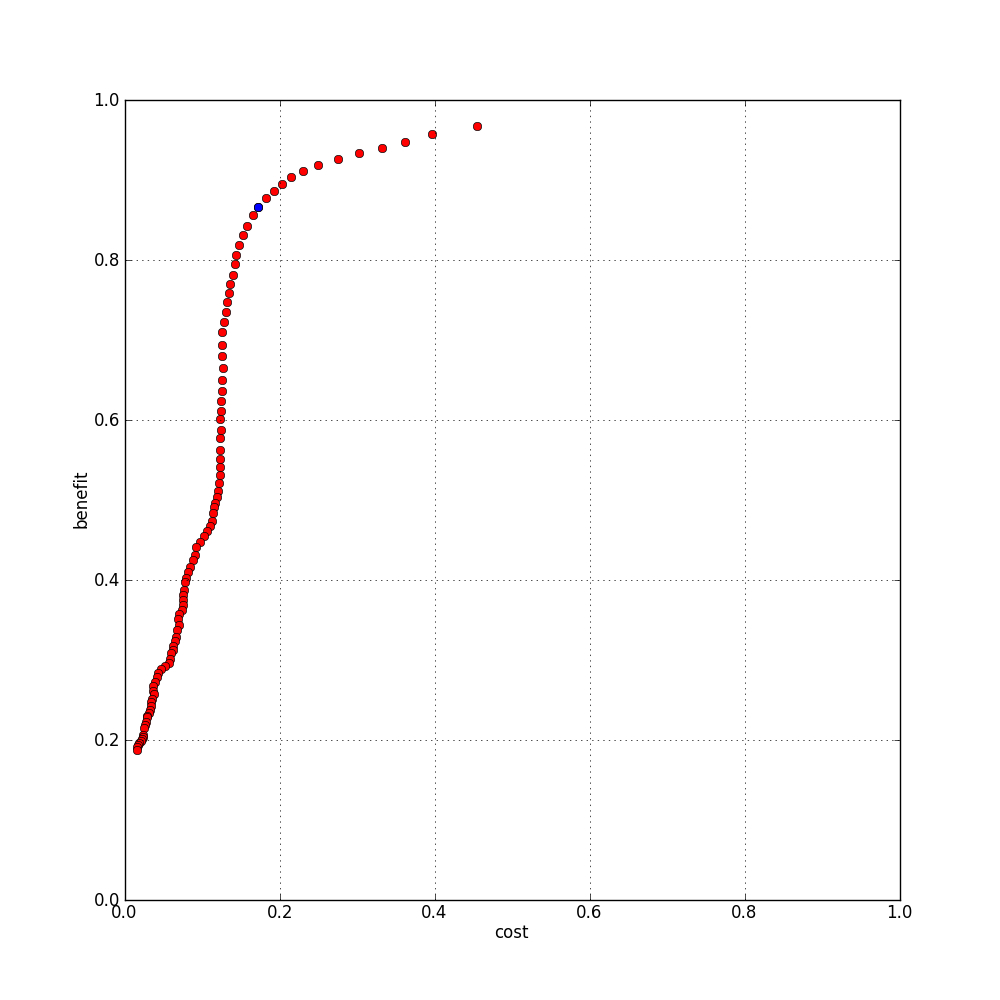
\includegraphics[width=0.75\textwidth]{img/2dcostbenefitexample2.jpg}
     \caption{An example of a 2D cost/benefit diagram, the blue configuration is the one with the lowest distance score}
\end{figure}
%
\subsubsection{Testing}
% ANDERS
For each algorithm, in each iteration of the 5-fold cross validation, we determine the optimal choice of parameter(s) and then use this configuration to classify the test-set. Obviously, we want the resulting distance-score to be as small as possible as this signifies a good performance, but we also try to capture some of the side-effects of the specific configuration. One of the things we are interrested in knowing is how many frames long the average good video-clip is. This in itself does not tell us much, since even a very good classifier could end up with very short video-clips if the footage it was classifying is very bad. However, if several algorithms perform equally well this could work as a tie-breaker, as we in general prefer long good-quality clips since they give us more room for manoeuvre later on when we have to actually segment the footage. The variance of this length along with the median lenght is also calculated.
%
\subsubsection{Robustness} \label{sec:robustness}
%
On top of the ordinary parameter tuning and testing we also attempt to measure the overall robustness of each of the algorithms with respect to the change of parameter. This is done by calculating the area under the curve (AUC) of the cost/benefit diagrams generated by each algorithm. For this we use the entire dataset, which is to say that it happens after the 5-fold cross validation. Any algorithm, whos benefit-value is generally larger than its corresponding cost-value, across all choices of parameter(s) will have an AUC larger than 0.5. The larger the AUC is the more robust the algorithm is toward changes to its parameter(s). Since the points produced by most of the algorithms are not evenly spread over the entire diagram, we insert points at the (0,0) and (1,1) coordinate in order to cover the entire span of the diagram along the x-axis. It can be argued whether this is the most correct way to handle this, but it does produce comparable AUCs across all algorithms. Unlike the tweaking and testing described above this does not tell us anything useful about the best parameter to choose since we have no way of knowing how this would generalise. But it does tell us something about the nature of the algorithm itself. In general we would prefer our algorithm of choice to be as robust as possible as it signifies a sensible selection of parameters. 
%
\subsubsection{Multi-parameter algorithms} \label{sec:ph1multiparameter}
%
All our algorithms, except one, only have one parameter. This makes them easy to tweak and test and also very straightforward to generate cost/benefit diagrams for. The \textit{ICSM} algorithm, however, has two parameters and this causes some problems. First and foremost the additional parameter makes tweaking much more computational expensive. With the other algorithms we tweak the one parameter by one percentage point in each iteration, which limits the number of configuration to a hundred. To do so with the \textit{ICSM} algorithm would require 10.000 tweak iterations, which is much too expensive even when the results of intermediate calculations are cached on disk. In order to bring this number down we start we start out by attempting to learn something about the base characteristics of the algorithm by probing it using some uniformly selected configurations. In the case of the \textit{ICSM} algorithm we see that the \textit{contrast} parameter has a huge influence on how well the algorithm is defined in the cost/benefit spectrum. For very low values of \textit{contrast} almost all results are undefined because all frames are marked as good, which makes it impossible to calculate precision and recall correctly. On the other end of the spectrum, when \textit{contrast} is large, the effect of changing it is very small, signifying that it converges toward some optimal value. Based on this information we choose to decrease the precision with which we tweak \textit{contrast} to ten percentage points per iteration. This brings the total number of tweak iterations down to 1000. This still takes a long time, but it is manageable.\\
\\
The second problem is encountered when generating the cost/benefit diagrams and calculating the AUC. The effect of changing more than one variable is not illustrated very well in a two-dimensional cost/benefit diagram. The points, which really belong in a higher dimensional space, are flattened into the plane resulting in several curves without any clear connection to each other. This also causes problems when calculating the AUC for the algorithm, since curves generated by bad performing configurations can be hidden below curves generated by good performing ones, which in the end results in a over-optimistic robustness score.
%
% \begin{figure}
%      \centering
%      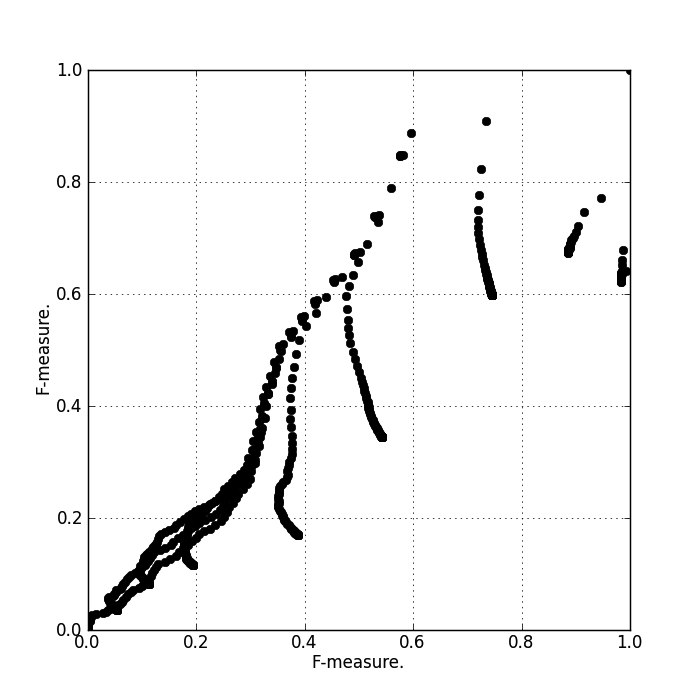
\includegraphics[width=0.75\textwidth]{img/2dcostbenefitexample.jpg}
%      \caption{An example of a 2D cost/benefit diagram for an algorithm with two variables}
% \end{figure}
%
%
% Noter fra Kim: Y-axis = benefit? X-axis=cost? Ser mærkeligt ud, drop!
%
In order to overcome this problem we simulate having only one parameter by locking the second one (contrast) to a specific value and then performing our analysis as usual. We repeat this over and over again, locking the contrast parameter to a new value in each iteration until we have covered all configuration combinations. For the robustness analysis we then add an aditional axis, representing the locked parameter, to our cost/benefit diagram and draw our points in three dimensions. The plane created illustrates the robustness of the algorithm much better. Since the choice of contrast values across all iterations are uniformly distributed, we can easily determine the AUC for the algorithm by simply calculating the individual AUCs for each selection of contrast value and compute an average.
%
\begin{figure}
     \centering
     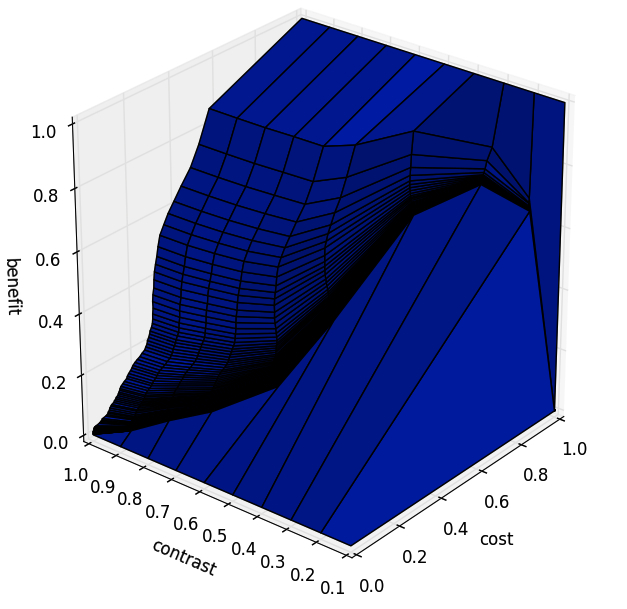
\includegraphics[width=0.75\textwidth]{img/3dcostbenefitexample.jpg}
     \caption{An example of a 3D cost/benefit diagram}
\end{figure}
%
\subsubsection{Test cases} \label{sec:testcases}
%
\paragraph{Frame by frame classification (FFC)}
%
The first test case only looks at each frame independently. For each frame we determine the level of contrast and the shift vector magnitude and use this information alone to perform a binary classification of the frame as \textit{good} or \textit{bad} using the algorithms described above. The results are compared with our \textit{gold standard} for the videos and the amount of true and false positives and negatives are used to calculate precision and recall for both classes.
%
\paragraph{Temporal classification (TC)} \label{sec:tctestcase}
%
In the second test case we change the way we punish misclassifications. We instead consider the videos as switching back and forth between two states, \textit{good} and \textit{bad}. Misclassifications, which happen close to these change-of-state's are punished less than those that happens elsewhere. The rationale behind this is that it is very difficult to objectively determine the exact point (frame) where a human observer will consider the quality of a video as changing from one state to the other. Likewise, we expect a human observer to ignore very short sub-parts of good or bad quality footage, if it is surrounded by a significant amount of footage of the opposite type. Overall, we want to be more tolerant of misclassifications, where it makes sense. For this we need a more advanced \textit{penalty function} than the simple binary check from the FFC test case.\\
%
We start by identifying all the positions in the sequence of frames where the state changes from good to bad or vice versa. Let $S$ be the set of all these positions. Also let $x$ any position in the video and let $c$ be some level of tolerance for mistakes. A \emph{penalty function} for determining the ratio of punishment for a misclassification at position $x$ is then defined as:
%
\begin{displaymath}
P(x) =1 - MAX_{s\in S}(e^{-\frac{(x-s)^{2}}{2c^{2}}})
\end{displaymath}
%
This function places a series of inverted gaussian bell curves at the point of every change of state. Figure \ref{fig:penaltycurve} shows an example of this. The value $c$ defines the width of the curve and thus determines how tolerant we are.
%
% Noter fra Kim: Valgt hvordan?
%
\begin{figure}
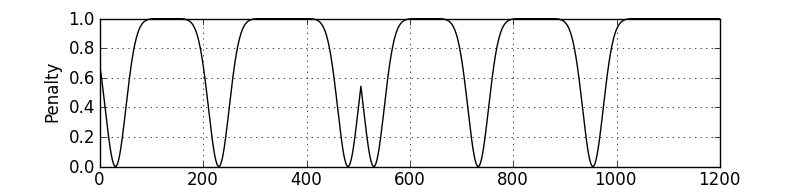
\includegraphics[width=1\textwidth]{img/penaltyfunction.jpg}
\caption{An illustration of a curve generated by the penalty function P}
\label{fig:penaltycurve}
\end{figure}
%
\emph{P(x)} always returns a value between 0 and 1, that tells us how severe a misclassification at position $x$ is. All correct classifications are treated just like in the FFC test case. However, if a misclassification occurs, we look at the \textit{penalty function} to see how the classification should be scored. There is one problem with this appraoch. It makes maintaining accurate true- and false- negative and positive values slightly less trivial. If a misclassification occurs at frame \textit{x} and \emph{P(x)} is very close to 0, how true (or false) is the classification)? The way we handle this is simply by adding \textit{P(x)} to the \textit{false} ratio for this type (positive or negative) and \textit{1 - P(X)} to the opposite type. That is, we quantify the classification as being both true and false to a varying degree determined by the \textit{penalty function}.
%
\paragraph{Smoothing of the algorithm suggestions}
%
Finally, for both algorithms, we also investigate the effect of smoothing the classification results. This is done to remove outliers in the final results and should not be confused with the smoothing of the \textit{contrast} and \textit{shift vector magnitudes} in the algorithms themselves.
%
\subsubsection{Results}
% ANDERS
In Table \ref{tab:algoconfigs} we have a number of different configurations of algorithms. The parameter is the average over the 5-fold cross validation. Smoothness degree describes how much the result is smoothed using triangular smoothing. The comparison method is either frame-by-frame (FFC) or temporal (TC), both described in section \ref{sec:testcases}.\\
%
\begin{table}
  \begin{tabular}{| l | l | p{2cm} | p{2cm} | c | c | }\hline
    Label & Algorithm & Smoothness degree & Comparison method & Tolerance & Parameter(s)\\\hline
    ICSM1 & ICSM & 0 & FFC & N/A & (0.052, 0.720) \\\hline
    ICSM2 & ICSM & 12 & FFC & N/A & (0.054, 0.720) \\\hline
    ICSM3 & ICSM & 0 & TC & 24 & (0.060,0.720) \\\hline
    ICSM4 & ICSM & 0 & TC & 48 & (0.064,0.720) \\\hline
    ICSM5 & ICSM & 12 & TC & 24 & (0.058,0.720) \\\hline
    ICSM6 & ICSM & 12 & TC & 48 & (0.064, 0.720) \\\hline
    ICSM7 & ICSM & 0 & TC & 12 & (0.056, 0.720) \\\hline\hline
%
    CCSM1 & CCSM & 0 & FFC & N/A & 0.092 \\\hline
    CCSM2 & CCSM & 12 & FFC & N/A & 0.088 \\\hline
    CCSM3 & CCSM & 0 & TC & 24 & 0.100 \\\hline
    CCSM4 & CCSM & 0 & TC & 48 & 0.108 \\\hline
    CCSM5 & CCSM & 12 & TC & 24 & 0.094 \\\hline
    CCSM6 & CCSM & 12 & TC & 48 & 0.110 \\\hline
    CCSM7 & CCSM & 0 & TC & 12 & 0.098 \\\hline\hline
%
    CO1 & CO & 0 & FFC & N/A & 0.462 \\\hline
    CO2 & CO & 12 & FFC & N/A & 0.460 \\\hline
    CO3 & CO & 0 & TC & 24 & 0.466 \\\hline
    CO4 & CO & 0 & TC & 48 & 0.474 \\\hline
    CO5 & CO & 12 & TC & 24 & 0.468 \\\hline
    CO6 & CO & 12 & TC & 48 & 0.474 \\\hline
    CO7 & CO & 0 & TC & 12 & 0.466 \\\hline\hline
%
    SO1 & SO & 0 & FFC & N/A & 0.048 \\\hline
    SO2 & SO & 12 & FFC & N/A & 0.048 \\\hline
    SO3 & SO & 0 & TC & 24 & 0.056 \\\hline
    SO4 & SO & 0 & TC & 48 & 0.060 \\\hline
    SO5 & SO & 12 & TC & 24 & 0.056 \\\hline
    SO6 & SO & 12 & TC & 48 & 0.060 \\\hline
    SO7 & SO & 0 & TC & 12 & 0.054 \\\hline\hline
%
    $\text{CSM}^{3}1$ & $\text{CSM}^{3}$  & 0 & FFC & N/A & 0.366 \\\hline
    $\text{CSM}^{3}2$ &$\text{CSM}^{3}$ & 12 & FFC & N/A & 0.366 \\\hline
    $\text{CSM}^{3}3$ &$\text{CSM}^{3}$ & 0 & TC & 24 & 0.370 \\\hline
    $\text{CSM}^{3}4$ &$\text{CSM}^{3}$ & 0 & TC & 48 & 0.388 \\\hline
    $\text{CSM}^{3}5$ &$\text{CSM}^{3}$ & 12 & TC & 24 & 0.370 \\\hline
    $\text{CSM}^{3}6$ &$\text{CSM}^{3}$ & 12 & TC & 48 & 0.382 \\\hline
    $\text{CSM}^{3}7$ &$\text{CSM}^{3}$ & 0 & TC & 12 & 0.370 \\\hline
%
  \end{tabular}
\caption{Algorithm configurations}
\label{tab:algoconfigs}
\end{table}
%
In Table \ref{tab:algoperf} the parameter(s) relative standard deviation is a measure of how much the parameter (is expected to) generalize to different data, where a low standard deviation equals a high level of generalization. The Distance Score (DS) is described in section \ref{sec:ph1tweaking}, and Area Under the Curve (AUC) is described in section \ref{sec:robustness}.\\
%
\begin{table}
  %\begin{tabular}{| l | p{2.5cm} |p{2.5cm} | p{2.5cm} | c |}\hline
  \begin{tabular}{| !l | ^p{2.5cm} | ^p{2.5cm} | ^p{2.5cm} | ^c |}\hline
    Label & Parameter(s) std. dev. \% & DS & DS std. dev. \% & AUC \\\hline
    ICSM1 & (7.7\%, 5.6\%) & 0.54 & 27.17\% & 0.51 (39.44\%) \\\hline
    CCSM1 & ~4.3\% & 0.54 & 27.90\% & 0.66 \\\hline
    CO1 & ~2.5\% & 0.81 & 28.10\% & 0.40 \\\hline
    SO1 & 15.6\% & 0.55 & 27.08\% & 0.65 \\\hline
    $\text{CSM}^{3}1$ & ~2.2\% & 0.76 & 30.27\% & 0.44 \\\hline\hline
%
    ICSM2 & (14.8\%, 5.6\%) & 0.54 & 27.52\% & 0.51 (39.69\%) \\\hline
    CCSM2 & 19.6\% & 0.54 & 27.85\% & 0.67 \\\hline
    CO2 & ~2.4\% & 0.81 & 28.21\% & 0.40 \\\hline
    SO2 & 15.6\% & 0.54 & 27.54\% & 0.65 \\\hline
    $\text{CSM}^{3}2$ & ~2.2\% & 0.76 & 30.87\% & 0.44 \\\hline\hline
%
    ICSM3 & (18.3\%, 5.6\%) & 0.29 & 31.10\% & 0.66 (41.71\%) \\\hline
    CCSM3 & 15.5\% & 0.30  & 34.30\% & 0.87  \\\hline
    CO3 & ~1.1\% & 0.50  & 28.73\% & 0.66 \\\hline
    SO3 & 14.3\% & 0.30  & 31.28\% & 0.86  \\\hline
    $\text{CSM}^{3}3$ & ~0.0\% & 0.45  & 31.90\% & 0.70 \\\hline\hline
%
    ICSM4 & (15.9\%, 5.6\%) & 0.21 & 34.29\% & 0.70 (42.57\%) \\\hline
    CCSM4 & 17.0\% & 0.22 & 34.24\% & 0.92 \\\hline
    CO4 & ~2.9\% & 0.39 & 18.54\% & 0.79 \\\hline
    SO4 & 18.3\% & 0.22 & 35.54\% & 0.91 \\\hline
    $\text{CSM}^{3}4$ & ~3.8\% & 0.36 & 20.37\% & 0.81 \\\hline\hline
%
    ICSM5 & (20.1\%, 5.6\%) & 0.29  & 32.02\% & 0.66 (41.78\%) \\\hline
    CCSM5 & 19.7\% & 0.30  & 33.81\% & 0.87  \\\hline
    CO5 & ~0.9\% & 0.49 & 28.31\% & 0.66 \\\hline
    SO5 & 14.3\% & 0.29 & 32.22\% & 0.86 \\\hline
    $\text{CSM}^{3}5$ & ~0.0\% & 0.45 & 32.62\% & 0.70 \\\hline\hline
%
    ICSM6 & (15.9\%, 5.6\%) & 0.21 & 35.18\% & 0.70 (42.62\%) \\\hline
    CCSM6 & 19.1\% & 0.22 & 35.00\% & 0.92 \\\hline
    CO6 & ~2.9\% & 0.40 & 18.65\% & 0.79 \\\hline
    SO6 & 18.3\% & 0.22 & 36.61\% & 0.91 \\\hline
    $\text{CSM}^{3}6$ & 18.3\% & 0.22 & 36.61\% & 0.91 \\\hline\hline
%
    ICSM7 & (14.3\%, 5.6\%) & 0.36 & 29.34\% & 0.62 (41.44\%) \\\hline
    \rowstyle{\bfseries}
    CCSM7 & 11.9\% & 0.36 & 31.71\% & 0.82 \\\hline
    CO7 & ~1.1\% & 0.60 & 26.18\% & 0.56 \\\hline
    SO7 & 14.8\% & 0.36 & 30.14\% & 0.81 \\\hline
    $\text{CSM}^{3}7$ & ~0.0\% & 0.55 & 28.93\% & 0.60 \\\hline
%
  \end{tabular}
\caption{Algorithm performance}
\label{tab:algoperf}
\end{table}
%
In Table \ref{tab:algoseq} a Good Sequence Length (GSL) is the number of consecutive good frames, and a Bad Sequence Length (BSL) is the number of consecutive bad frames. Both measures is an average (over each test-set) and the relative standard deviation along with the longest GSL and BSL is also supplied in Table \ref{tab:algoseq}.
%
\begin{table}
  \begin{tabular}{| l | c | c | c | c | c | c |}\hline
  %\begin{tabular}{| !l | ^c | ^c | ^c | ^c | ^c | c |}\hline
    Label & GSL & GSL std. dev. \% & longest GSL & BSL & BSL std. dev. \% & longest BSL  \\\hline
    ICSM1 & 205 & 217\% & 5105 & 40 & 155\% & 536 \\\hline
    CCSM1 & 214 & 214\% & 5121 & 40 & 160\% & 607 \\\hline
    CO1 & 290 & 28\% & 11079 & 73 & 196\% & 1690 \\\hline
    SO1 & 198 & 221\% & 5105 & 40 & 157\% & 743 \\\hline
    $\text{CSM}^{3}1$ & 264 & 326\% & 11078 & 69 & 204\% & 1691 \\\hline\hline
%
    ICSM2 & 248 & 199\% & 5115 & 47 & 152\% & 608 \\\hline
    CCSM2 &245 & 200\% & 5118 & 47 & 164\% & 739 \\\hline
    CO2 & 328 & 317\% & 11079 & 84 & 185\% & 1718 \\\hline
    SO2 & 231 & 206\% & 5115 & 47 & 170\% & 1087 \\\hline
    $\text{CSM}^{3}2$ & 309 & 301\% & 11078 & 80 & 190\% & 1692 \\\hline\hline
%
    ICSM3 & 221 & 210\% & 5105 & 39 & 156\% & 509 \\\hline
    CCSM3 & 222 & 210\% & 5121 & 39 & 162\% & 607 \\\hline
    CO3 & 340 & 308\% & 11079 & 69 & 215\% & 1690 \\\hline
    SO3 & 209 & 214\% & 5105 & 38 & 147\% & 491 \\\hline
    $\text{CSM}^{3}3$ & 319 & 298\% & 11078 & 66 & 223\% & 1691 \\\hline\hline
%
    ICSM4 & 229 & 209\% & 5122 & 39 & 149\% & 509 \\\hline
    CCSM4 & 225 & 213\% & 5123 & 38 & 154\% & 537 \\\hline
    CO4 & 378 & 316\% & 12080 & 71 & 217\% & 1690 \\\hline
    SO4 & 216 & 209\% & 5122 & 37 & 147\% & 482 \\\hline
    $\text{CSM}^{3}4$ & 388 & 280\% & 12082 & 59 & 225\% & 1687 \\\hline\hline
%
    ICSM5 & 257 & 186\% & 5115 & 47 & 149\% & 608 \\\hline
    CCSM5 & 248 & 198\% & 5118 & 46 & 156\% & 739 \\\hline
    CO5 & 411 & 290\% & 11079 & 80 & 202\% & 1690 \\\hline
    SO5 & 246 & 200\% & 5115 & 45 & 143\% & 608 \\\hline
    $\text{CSM}^{3}5$ & 364 & 280\% & 11078 & 75 & 211\% & 1692 \\\hline\hline
%
    ICSM6 & 266 & 198\% & 5122 & 45 & 144\% & 534 \\\hline
    CCSM6 & 260 & 200\% & 5129 & 45 & 142\% & 537 \\\hline
    CO6 & 431 & 298\% & 12080 & 82 & 201\% & 1690 \\\hline
    SO6 & 259 & 195\% & 5122 & 45 & 139\% & 482 \\\hline
    $\text{CSM}^{3}6$ & 397 & 284\% & 12082 & 74 & 215\% & 1687 \\\hline\hline
%
    ICSM7 & 212 & 213\% & 5105 & 39 & 153\% & 510 \\\hline
    CCSM7 & 220 & 212\% & 5121 & 39 & 162\% & 607 \\\hline
    CO7 & 340 & 308\% & 11079 & 69 & 215\% & 1690 \\\hline
    SO7 & 208 & 214\% & 5105 & 39 & 149\% & 491 \\\hline
    $\text{CSM}^{3}7$ & 319 & 298\% & 11078 & 66 & 223\% & 1691 \\\hline
  \end{tabular}
\caption{Sequence data}
\label{tab:algoseq}
\end{table}
%
\subsubsection{Analysis of results}
%
Table \ref{tab:algoperf} summarizes the primary results of our test. We cannot directly compare different configurations of the various algorithms as we expect a higher tolerance for error in some configurations, either by applying a gaussian filter (as described in Section [REFERENCE]) in the comparison method or triangular smoothing (as described in Section [REFERENCE]) of the result, or both.\\
We therefore try to identify the configuration with the best performance mainly by comparing distance scores (low is better). Secondly the generalizability of a configuration is taken into account to break ties by looking at the relative standard deviation of the parameter(s).\\
AUC is also mentioned in the table, but as it describes how sensitive an algorithm is to parameter-change...\\
We did not expect the CO\textit{X} and $\text{CSM}^{3}\textit{X}$ algorithms to perform very well as the first does not take camera-movement into account, and the second ???????????????????????\\
The 7th configuration does not apply triangular smoothing, and also uses a fairly low tolerance of 12 frames, roughly translated to a margin of error of half a second in each end of a sequence, yet it still achives a distance score of $0.36$ in 3 out of 5 algorithms and a relative standard deviation around $30\%$. We use the parameter relative standard deviation to break the tie where CCSM7 comes out on top. It also has the highest AUC, and we should therefore expect it to perform well even for other choices of parameters.\\
The performance can generally be explained by the nature of our dataset, as there simply is very few frames where contrast is an issue. The higher relative standard deviation of SO7 could be explained by it trying to overcompensate in the few cases where a frame is classified as bad because of a low contrast.
%
\subsubsection{Analysis risks}
% LAUGE
In order to limit the scope of the testing and analysis phase we make some decisions which should be noted as a lot of areas related to determining the best algorithm and the optimal algorithm-parameter combination are left to be explored:\\
\\
All our algorithms square the \textit{contrast} and \textit{shift vector magnitude} values they come up with for each frame. The reason for this is that we want to increase their sensitivity toward bad values as compared to good ones. However, we have not done any real experimentation in this context and it is possible that a higher or lower power would yield better results. Furthermore we smooth these values across neighbouring frames in order to eliminate the worst outliers. It does not seem to have any significant effect on the final correctness of the algorithms, but this is neither an area in which we have done any real experimentation. Another important thing to remember is that we actually compute \textit{contrast} differently than Girgensohn et al. \cite{Girgensohn:2000:SAH:354401.354415}. Our method should be more robust toward very uniformly colored frames, but their original method could be more effective in general.\\
\\
When generating the cost and benefit scores we calculate the harmonic mean between the positive precision and the negative recall, as well as the positive recall and the negative precision, respectively. In our experimentation we have simply weighted the two values in each pair evenly, but it is possible that a skewed weighting in one or both of means would perform differently. It is even possible that this pair combination is not the right one for the task, although we argue that it intuitively makes sense.\\
\\
In our experiment with smoothing the classification suggestions generated by the algorithm, in order to remove outliers, we restrict ourselves to only testing two different degrees of smoothing. More could be learned by experimenting with this value as an additional parameter of the algorithms.\\
\\
The same can be said about the tolerance-value in the Temporal Classification test case (page ~\pageref{sec:tctestcase}). Exactly what degree of tolerance is the most reasonable is up for debate and any changes could, and probably would, change the outcome of our results.\\
\\
Also mentioned ealier, when calculating the AUC's for each algorithm we insert the points (0,0) (1,1) along with the points generated by the cost/benefit calculations in order to make sure each algorithm's curve cover the entire span of the x-axis. This has the effect of normalising the AUC around 0.5, which is useful for AUCs based on a curve that is only defined partly along the x-axis. It is however possible, that the very fact that a curve is not defined all along the x-axis is a sign of low robustness especially if the curve only is present near x = 1, that is, if the cost value is generally very high. If this is the case we risk ending up with invalid assumptions of robustness.\\
\\
In the \textit{ICSM} algorithm we chose to simplify our tweaking process by decreasing the precision on the second parameter, \textit{contrast}. The rationale for this is described in section~ \ref{sec:ph1multiparameter} on page ~\pageref{sec:ph1multiparameter}. This means that our understanding of the influence of contrast in this algorithm is less detailed.\\
\\
Finally, it should be mentioned that all our tests are performed by treating the quality assessment problem as a task of binary classification. As described in section~ \ref{sec:videoclipsegmentation} on page ~\pageref{sec:videoclipsegmentation}, we are actually not interested in such a hard classification in the final system. Rather we want the quality of a region of video-footage to be expressed as a soft (un)suitability curve, from which we can make some general assumptions. However, the nature of our tests, especially the way in which we generate our gold standard (section~ \ref{sec:framequalityassessmentdataset} on page ~\pageref{sec:framequalityassessmentdataset}), requires us to simplify the problem into this binary form. Some of the aspects of the problem, which are lost by doing this, are to some extent accounted for, for example in the Temporal Classification test case (page ~\pageref{sec:tctestcase}), which allows for misclassifications to be treated in a more soft manner, but others are undeniably lost. This should also be taken into account, when considering the generalisability of our results.
%
\subsection{Section summary}
%
We have explored different methods for estimating the image quality in video footage. Our approach focuses on the overall level of contrast in the individual frames as well as the movement of the camera. We have constructed, and testet, a set of algoritms, which uses these two variables to compute an unsuitability score for each frame in the videos. This score is then cast into the binary range using configurable threshold values. We compare the different algorithms 